\documentclass{beamer}
\usepackage{beamerthemeshadow}
\usepackage{beamerthemeDarmstadt}
\usepackage{multicol}
%\usepackage{pgfpages}
%\pgfpagesuselayout{resize to}[letterpaper,border shrink=5mm,portrait]

% \usepackage[english]{babel}
% \usepackage[latin1]{inputenc}
% \usepackage{times}
% \usepackage[T1]{fontenc}
% \usepackage{graphicx,subfigure}
% \usepackage{color}
% \usepackage{amsmath}
% 


% user's definition

\newenvironment{changemargin}[2]{%
  \begin{list}{}{%
    \setlength{\topsep}{0pt}%
    \setlength{\leftmargin}{#1}%
    \setlength{\rightmargin}{#2}%
    \setlength{\listparindent}{\parindent}%
    \setlength{\itemindent}{\parindent}%
    \setlength{\parsep}{\parskip}%
  }%
  \item}{\end{list}}

\title[Predicting The Stock Market With Deep Learning]
{\ Predicting The Stock Market With Deep Learning}


\author{Michael Holmblad}

\date{4/29/2020}

\institute[VU] {Villnanova University}



%-------------------------------------------------------------------
\begin{document}

\begin{frame}
  \titlepage 
\end{frame}



%---------------------------------------------------
\section{Intro}
\subsection{}
\frame{{Introduction}
 \begin{itemize}
 	\item<1->Predicting the stock market?
 	\item<2->Deep Learning and prediction
 	\item<3->Can deep learning be a tool to solve it? 
 \end{itemize}
}

\frame{{History}
	\begin{itemize}
		\item<1->Stock market prediction goes at least back to the 60s 
		\item<2->Data processing issues, back propagation attempt 
		\item<3->Simulating 
	\end{itemize}
}

\section{Buildup}
\subsection{S\&P 500}
\frame{{S\&P 500 Data}
	\begin{itemize}
		\item<1->Composes of over 80\% of the American stock market
		\item<2->Popular for usage in stock prediction studies
		\item<3->Everything is in the form of time series data
	\end{itemize}	
}

\frame{{Event Based Prediction}
	\begin{itemize}
		\item<1->Open IE combined with a simple neural network 
		\item<2->Expansion with Neural Tensor Networks and a CNN
		\item<3->Common practice for event based prediction
	\end{itemize}	
}

\frame{{Results}
	\begin{figure}[h]
		\centering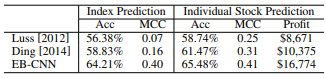
\includegraphics[width=3in]{textSeriesResults}
		\caption{(Ding et al, 2015)}
	\end{figure}
}

\frame{{Corporate and Education Realm}
	\begin{itemize}
		\item<1->The Private sector mainly used linear models for predicting the stock market
		\item<2->Auto Regressive Integrated Moving Average was the standard
		\item<3->Google and other companies teamed up with universities like Stanford to test LSTMs 
	\end{itemize}
}

\subsection{FI-2010}
\frame{{Limit Order Books}
	\begin{itemize}
		\item<1->A record of outstanding limit orders maintained by the security specialist who works at the exchange
		\item<2->The FI-2010 dataset, NASDAQ Nordic benchmark dataset 
		\item<3->Popular for testing European stock market prediction
	\end{itemize}
}

\frame{{CNN and LSTM Combinations}
	\begin{figure}[h]
		\centering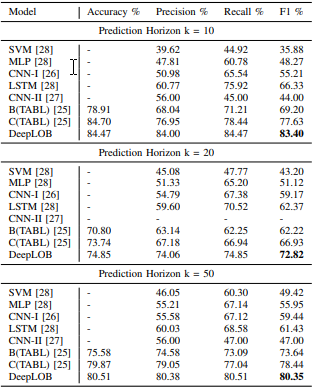
\includegraphics[width=2in]{fi2010}
		\caption{(Passalis et al., 2018)}
	\end{figure}
}

\section{Standouts}
\subsection{ }
\frame{{Deep ConvLSTM Project}
	\begin{figure}[h]
		\centering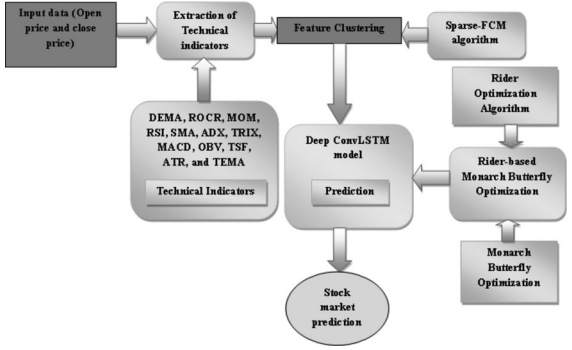
\includegraphics[width=3in]{butterfly}
		\caption{(Kelotra, 2020)}
	\end{figure}
}

\frame{{Reinforcement Learning}
	\begin{figure}[h]
		\centering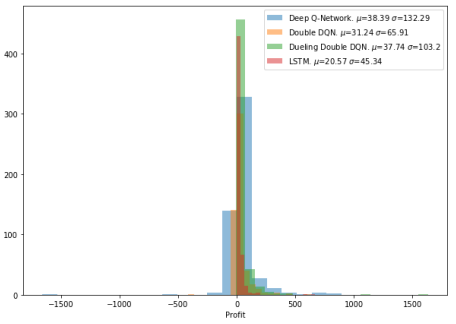
\includegraphics[width=3in]{rlstock}
		\caption{(Dang, 2019)}
	\end{figure}
}

\section{Conclusion}
\subsection{}
\frame{{What We've Learned}
	\begin{itemize}
		\item<1->A lot closer to understanding stock market prediction
		\item<2->Feature Extraction
		\item<3->Best at doing this task
	\end{itemize}
}

\frame{{Future Work}
	\begin{itemize}
		\item<1->Triple check dates, website citations
		\item<2->Try implementing these kind of models
		\item<3->Track how popular the 2019/2020 papers become
	\end{itemize}
}
\frame{{Resources}
 \centering Holmblad, Michael. Survey of Deep Learning and Stock Market Prediction
}
\frame{{Questions?}
	\center
\includegraphics[width=2.5in]{questionpicture.jpeg}
}
\end{document}
